%%%%%%%%%%%%%%%%%%%%%%%%%%%%%%%%%%%%%%%%%%%%%%%%%%%%%%%%%%%%%%%%%%%%
%%
%%                     Materiais
%%
%%%%%%%%%%%%%%%%%%%%%%%%%%%%%%%%%%%%%%%%%%%%%%%%%%%%%%%%%%%%%%%%%%%%

    \begin{frame}{Materiais}
       \begin{figure}[!ht]
        \centering % para centralizar a figur
          %
          \begin{subfigure}[H]{0.3\textwidth}
            
\includegraphics[width=\textwidth]{img/logo/Python.png}
            \label{fig_op_ag}
          \end{subfigure}
          \hspace*{0.80cm}
          \begin{subfigure}[H]{0.2\textwidth}
            
\includegraphics[width=\textwidth]{img/logo/OpenCv.png}
            \label{fig_op_af}
          \end{subfigure}
          \hspace*{0.80cm}
          \begin{subfigure}[H]{0.3\textwidth}
            
\includegraphics[width=\textwidth]{img/logo/MediaPipe.png}
            \label{fig_op_af}
          \end{subfigure}
          \begin{subfigure}[H]{0.3\textwidth}
            
\includegraphics[width=\textwidth]{img/logo/Git.png}
          \end{subfigure}
          
      
    \end{figure}
\end{frame}


%%%%%%%%%%%%%%%%%%%%%%%%%%%%%%%%%%%%%%%%%%%%%%%%%%%%%%%%%%%%%%%%%%%%
%%
%%                     Método
%%
%%%%%%%%%%%%%%%%%%%%%%%%%%%%%%%%%%%%%%%%%%%%%%%%%%%%%%%%%%%%%%%%%%%%

\begin{frame}{Método}
    \begin{enumerate}
        \item Realização de revisão da literatura abordando o uso de visão computacional associado ao treinamento físico.
        \vspace*{0.80cm}
        \item Escolha das tecnologias.
        \vspace*{0.80cm}
        \item Criação de uma estrategia para deteção do movimento correto de barra fixa
        \vspace*{0.80cm}
        \item Desenvolvimento de uma Ferramenta computacional para detecção da execução correta da barra fixa.
    \end{enumerate}
\end{frame}


\begin{frame}{Método}
    \begin{figure}[!ht]
        \centering
        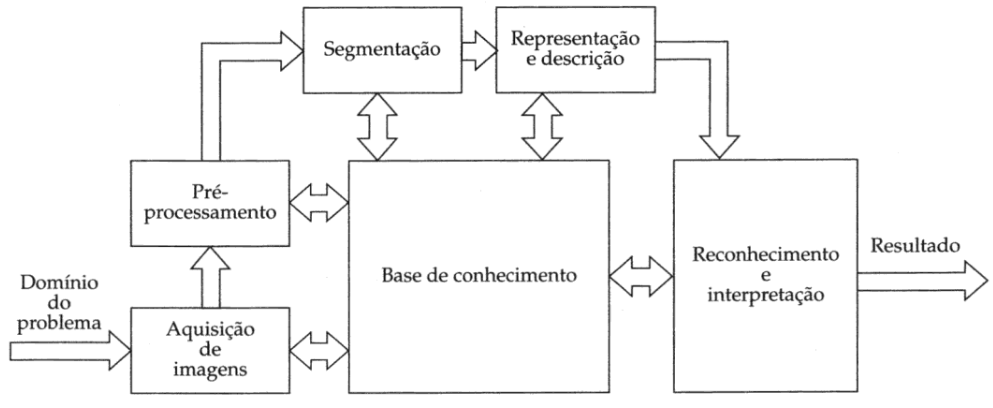
\includegraphics[scale=0.33]{img/metodos/processamentoImagem.png}
        \caption*{(GONZALEZ; WOODS, 2000)}
    \end{figure}
\end{frame}